\setchapterpreamble[u]{\margintoc}
\chapter{Network security endpoint}
\labch{chapter7}


\section{Firewall}

Tipicamente inserito tra la rete e Internet o all'interno della rete per isolarne delle porzioni. 

Scopo:  creare un perimetro esterno di sicurezza che protegga la rete dagli attacchi tramite internet, fornire un unico punto dove settare sicurezza e auditing, isolare sezioni della rete dalla rete stessa o dall'esterno.

Funzionamento ad alto livello: 
\begin{itemize}
    \item Tutto il traffico dall'interno verso l'esterno, e viceversa, passa attraverso il firewall. Ciò si ottiene bloccando fisicamente tutti gli accessi alla rete locale eccetto tramite il firewall;
	\item Solo il traffico autorizzato, come definito dalla security policy locale, può passare. Diversi tipi di firewall possono usare diversi tipi di policy;
	\item Il firewall stesso deve essere immune alla penetrazione. Ciò implica l'uso di un sistema rinforzato con un sistema operativo protetto. I sistemi informatici affidabili sono adatti per ospitare un firewall e sono spesso richiesti nelle applicazioni governative.
\end{itemize}

Tecniche utilizzate dai firewall per controllare l'accesso e applicare la politica di sicurezza decisa:
\begin{itemize}
    \item Controllo sul servizio: determina i tipi di servizi Internet che possono essere accessibili, in entrata o in uscita (posso avere policy diverse per entrata e uscita);
	\item Controllo sulla direzione: determina la direzione in cui le richieste di un particolare servizio possono essere avviate e consentite a fluire attraverso il firewall;
	\item Controllo sull'utente: controlla l'accesso a un servizio in base a quale utente sta tentando di accedervi;
	\item Controllo sul comportamento: controlla come vengono utilizzati determinati servizi.
\end{itemize}

Funzionalità:
\begin{itemize}
    \item Un firewall definisce un unico punto di strozzatura che tiene gli utenti non autorizzati fuori dalla rete protetta, impedisce a servizi potenzialmente vulnerabili di entrare o uscire dalla rete e fornisce protezione da vari tipi di attacchi IP spoofing e di routing;
	\item Un firewall fornisce una posizione per il monitoraggio di eventi relativi alla sicurezza (audit, allarmi, ecc.);
	\item Un firewall è una piattaforma conveniente per diverse funzioni Internet non correlate alla sicurezza (NAT, log sull'uso di internet, …);
	\item Un firewall può fungere da piattaforma per l'implementazione di virtual private network.
\end{itemize}

Limiti del firewall:
\begin{itemize}
    \item  Il firewall non può proteggere da attacchi che aggirano il firewall;
	\item Il firewall potrebbe non proteggere completamente dalle minacce interne, come un dipendente scontento o un dipendente che collabora inconsapevolmente con un aggressore esterno;
	\item È possibile accedere a una wireless LAN protetta in modo non corretto dall'esterno dell'organizzazione. Un firewall interno che separa porzioni della rete aziendale non può proteggere dalle comunicazioni wireless tra sistemi locali su lati diversi del firewall interno;
	\item Il firewall non può proteggere da dispositivi infettati fuori dalla rete aziendale che vengono successivamente connessi e usati.
\end{itemize}

\subsection{Firewall packet filter}

\begin{figure}[h]
    \centering
    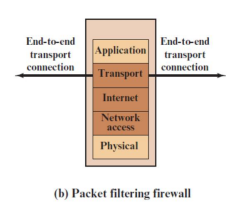
\includegraphics[width=1\textwidth]{images/chapter7/7-1.png}
    \caption{Reti wireless.}
    \label{fig:7-1}
\end{figure}

Esamina tutti i tipi di pacchetti di dati in entrata o in uscita in esecuzione sulla rete, verificando: 
\begin{itemize}
    \item Origine del pacchetto;
	\item Destinazione del pacchetto;
	\item Porta di origine e destinazione.
\end{itemize}

Quando i pacchetti superano il processo di ispezione, il firewall consente ai pacchetti di entrare nella rete o nel dispositivo. I pacchetti che non riescono a passare vengono bloccati.
Solitamente definisco le configurazioni di entrata/usciti consentite (più specifiche configurazioni non consentite) e blocco tutto il resto.

Vantaggi: semplicità, velocità, trasparente agli utenti.

Svantaggi:
\begin{itemize}
    \item Non possono impedire attacchi che impiegano vulnerabilità o funzioni delle applicazioni;  
	\item Limitate funzionalità di log (indirizzo IP, porte, tipo di traffico, flag,..);
	\item La maggior parte di questi firewall non supporta user authentication avanzate;
	\item Sono generalmente vulnerabili ad attacchi e exploit che sfruttano i problemi all'interno della specifica TCP/IP e dello stack di protocollo;
	\item Sono suscettibili a violazioni alla sicurezza causate da configurazioni improprie.
\end{itemize}

Attacchi e contromisure:
\begin{itemize}
    \item Spoofing dell'indirizzo IP: l'attaccante trasmette i pacchetti dall'esterno usando come indirizzo IP di origine l'indirizzo di un host interno (mi spaccio per un altro indirizzo IP);
	\begin{itemize}
	    \item La contromisura è scartare i pacchetti con un indirizzo di origine interno se arriva su un'interfaccia esterna (non ha senso che un pacchetto inviato da un host interno alla rete arrivi da fuori la rete). Questa contromisura è spesso implementata al router esterno al firewall.
	\end{itemize}
	\item Source routing attack: la stazione di origine specifica il percorso che un pacchetto dovrebbe seguire mentre attraversa Internet, nella speranza che ciò aggiri il firewall;
	\begin{itemize}
	    \item La contromisura consiste nell'eliminare tutti i pacchetti che lo utilizzano questa opzione.
	\end{itemize}
	\item Tiny fragment attacks: l'intruso utilizza l'opzione di frammentazione IP per creare frammenti estremamente piccoli e forzare le informazioni dell'header TCP in un frammento di pacchetto separato.
	\begin{itemize}
	    \item La contromisura consiste nell'usare una regola per cui il primo frammento di un pacchetto deve contenere una quantità minima di info sull'header del protocollo di trasporto. Se il primo frammento viene rifiutato, il filtro può ricordare il pacchetto ed eliminare tutti i frammenti successivi;
		\item Posso oppure scartare direttamente i pacchetti che usano al flag di frammentazione.
	\end{itemize}
\end{itemize}

\subsection{Firewall statefull inspection}

\begin{figure}[h]
    \centering
    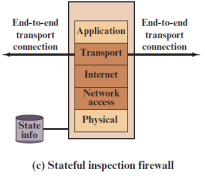
\includegraphics[width=1\textwidth]{images/chapter7/7-2.png}
    \caption{Reti wireless.}
    \label{fig:7-2}
\end{figure}

\begin{itemize}
    \item Monitora lo stato delle connessioni (tipo di connessione e porta) attive e utilizza tali informazioni per consentire ai pacchetti di rete di attraversare il firewall;
	\item L'esterno può inviare quell'informazione solo su quella connessione, quindi solo a quella porta di quell'host;
	\item Questi firewall, a volte, possono andare anche a controllare il sequence number del pacchetto TCP, per evitare attacchi di replay;
    \item Versione rinforzata dei packet-filter.
\end{itemize}

\subsection{Application-Level Gateway}

\begin{figure}[h]
    \centering
    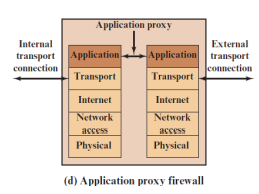
\includegraphics[width=1\textwidth]{images/chapter7/7-3.png}
    \caption{Reti wireless.}
    \label{fig:7-3}
\end{figure}

\subsection{Circuit-level gateway}

\begin{figure}[h]
    \centering
    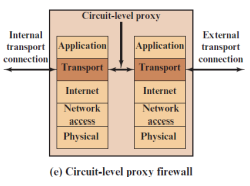
\includegraphics[width=1\textwidth]{images/chapter7/7-4.png}
    \caption{Reti wireless.}
    \label{fig:7-4}
\end{figure}

\begin{itemize}
    \item Può essere un sistema autonomo o può essere una funzione specializzata eseguita da un gateway a livello di applicazione per determinate applicazioni:
	\item Non consente una connessione TCP end to end. Si basa su due connessioni, ciascuna delle quali può avere policy diverse;
	\item La funzione di sicurezza determina quali connessioni sono consentite;
	\item Una tipica situazione d'uso è quando l'amministratore del sistema di fida degli utenti interni.
\end{itemize}

Un bastion host è un host rafforzato dal punto di vista della sicurezza (hardened OS, servizi essenziali, autenticazione rafforzata, …) che runna il circuit-level gateway ed è solitamente la prima macchina esposta su Internet.

\begin{figure}[h]
    \centering
    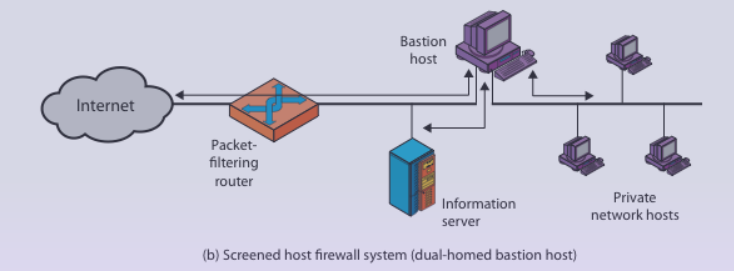
\includegraphics[width=1\textwidth]{images/chapter7/7-5.png}
    \caption{Reti wireless.}
    \label{fig:7-5}
\end{figure}

\subsection{DMZ (Demilitarised Zone)}

Si riferisce a una rete appositamente controllata situata tra la rete esterna (Internet) e la rete interna. Rappresenta una sorta di zona cuscinetto che separa le reti da rigide regole di comunicazione e firewall. L'area demilitarizzata contiene server quali server Web, server di posta, server di autenticazione o gateway applicazione. Solo questi sono accessibili agli utenti da Internet. Separando la DMZ dalla rete interna, gli utenti esterni non possono accedere alle risorse interne. La rete privata rimane protetta dagli attacchi provenienti da Internet o dal sovraccarico delle richieste Internet. La zona demilitarizzata può essere separata dalle reti adiacenti da uno o più firewall, che proteggono sia in ingresso che in uscita.

\begin{figure}[h]
    \centering
    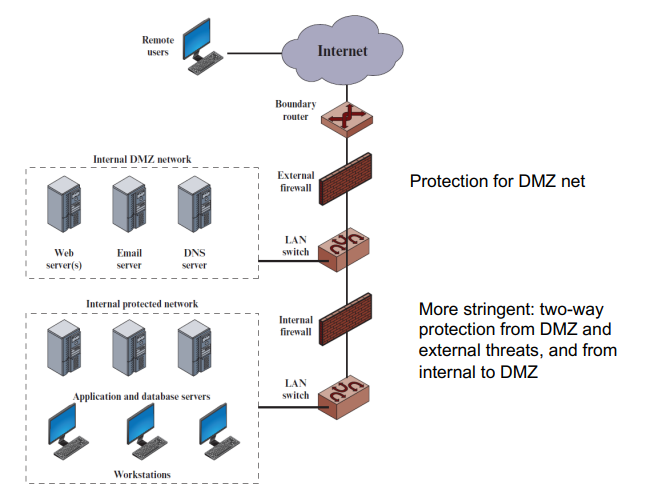
\includegraphics[width=1\textwidth]{images/chapter7/7-6.png}
    \caption{Reti wireless.}
    \label{fig:7-6}
\end{figure}

\section{Intrusion Detection System}

Concetti base:
\begin{itemize}
    \item Intrusioni: violazioni delle policy di sicurezza, generalmente caratterizzate come tentativi di intaccare la riservatezza, l'integrità o la disponibilità di un computer o di una rete. Queste violazioni possono provenire da aggressori che accedono ai sistemi da Internet o da utenti autorizzati dei sistemi che tentano di superare i loro legittimi livelli di autorizzazione o che utilizzano il loro legittimo accesso al sistema per condurre attività non autorizzate;
	\item Detection dell'intruzione: processo di raccolta delle informazioni sugli eventi che si verificano in un sistema o rete e la loro analisi alla ricerca di segni dell'intruzione;
	\item Intrusione detection system: prodotti hardware o software che raccolgono e analizzano informazioni da varie aree all'interno di un computer o una rete allo scopo di trovare e fornire avvisi in tempo reale o quasi in tempo reale di tentativi di accesso alle risorse di sistema in modo non autorizzato.
\end{itemize}

Possono essere classificati in:
\begin{itemize}
    \item Host-based IDS: monitora le caratteristiche di un singolo host e gli eventi che si verificano all'interno di tale host per attività sospette;
	\item Network-based host: monitora il traffico di rete per particolari segmenti di rete o dispositivi e analizza la rete, il trasporto e i protocolli applicativi per identificare attività sospette.
\end{itemize}

Componenti logiche:
\begin{itemize}
    \item Sensori: sono responsabili della raccolta dei dati. L'input per un sensore può essere qualsiasi parte di un sistema che potrebbe contenere prove di un'intrusione. I tipi di input per un sensore includono pacchetti di rete, file di log e tracce delle chiamate di sistema. I sensori raccolgono e inoltrano queste informazioni all'analizzatore;
	\item Analizzatore: ricevono input da uno o più sensori o da altri analizzatori. L'analizzatore è responsabile di determinare se si è verificata un'intrusione. L'output di questo componente indica che si è verificata un'intrusione. L'output può includere prove a sostegno della conclusione che si è verificata un'intrusione. L'analizzatore può fornire indicazioni sulle azioni da intraprendere a seguito dell'intrusione;
	\item Interfaccia utente: consente all'utente di visualizzare l'output del sistema o di controllare il comportamento del sistema. In alcuni sistemi, l'interfaccia utente può equivalere a un componente manager, director o console.
\end{itemize}

Approcci all'intrusion detection:
\begin{itemize}
    \item Misuse (abusi) detection: definisco delle regole di pattern di attacco. Se questi pattern si verificano allora sono sotto attacco. Ho pochi falsi positivi, ma non riconosco attacchi che non seguono i pattern che ho inserito (faccio un profilo dell'attaccante);
	\item Anomaly detection: ricerco attività anomale secondo alcuni criteri sul corretto comportamento del sistema. Può rilevare attacchi nuovi e sconosciuti, ma può generare falsi positivi/negativi (faccio un profilo sul sistema).
\end{itemize}

IDS basato su host:
\begin{itemize}
    \item Aggiunge un layer specializzato sulla sicurezza sw a sistemi vulnerabili o sensibili;
	\item Monitora le attività nel sistema in più modi per cercare comportamenti sospetti;
	\item In alcuni casi può stoppare un attacco prima che il danno venga fatto, anche se il suo compito principale resta individuare le intrusioni, loggare eventi sospetti e lanciare allarmi;
	\item Può individuare intrusioni interne e esterne;
	\item Può basarsi sulla misuse protection, anomaly protection o una combinazione di entrambe. Per l'anomaly detection, 2 strategia comuni sono:
	\begin{itemize}
	    \item Threshold detection: controllo delle soglie, come quante connessioni sto creando in parallelo, …;
		\item Profiled based: creo uno storico sul comportamento dell'utente e faccio delle stime. 
	\end{itemize}
\end{itemize}

IDS basato sulla rete (NIDS):
\begin{itemize}
    \item Monitora il traffico sul suo segmento di rete come fonte di dati, settando le interfacce delle schede di rete in modo promiscuo per catturare tutto il traffico che passa per il suo segmento di rete;
	\item Il traffico di rete sugli altri segmenti deve essere controllato da altri NIDS;
	\item Controlla i pacchetti sulla rete nel momento in cui passano per qualche sensore. Un pacchetto viene considerato se matcha una certa firma. I tipi di firma sono:
	\begin{itemize}
	    \item Stringa: cerca una strigna di testo che indica un possibile attacco;
		\item Porta: controlla tentativi di connessione a porte che sa essere attaccate frequentemente;
		\item Condizione sull'header: controlla alla ricerca di combinazioni di header illefali o pericolose.
	\end{itemize}
	\item Posso piazzare i suoi sensori in 4 punti principali della rete, per segmentarla:
	\begin{itemize}
	    \item All'ingrasso della rete;
		\item Al livello della DMZ;
		\item Al livello delle parti più importanti delle rete interna;
		\item Al livello degli host, per monitorare lo workstation.
	\end{itemize}
\end{itemize}

\begin{figure}[h]
    \centering
    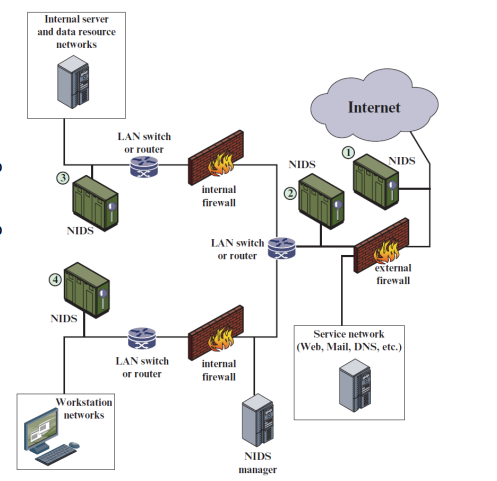
\includegraphics[width=1\textwidth]{images/chapter7/7-7.png}
    \caption{Reti wireless.}
    \label{fig:7-7}
\end{figure}